\documentclass[12pt,twocolumn]{report}
\usepackage{amsfonts}
\usepackage{amsmath}
\usepackage{tikz}
\usepackage{pgfplots}
\usepackage{ngerman}

\pgfplotsset{compat=1.18}

\title{Das Diffie-Hellman Verfahren}
\author{Tim Teichmann}
\date{\today}

\begin{document}
\maketitle

\section*{Funktionsweise}
\begin{flushleft}
Alice und Bob möchten sicher miteinander kommunizieren.
Das funktioniert indem sie einen gemeinsamen Schlüssel bestimmen,
mit dem sie ihre Nachrichten verschlüsseln können. Dieser gemeinsame
Schlüssel sollte nur den beiden bekannt sein.

Um sicher einen gemeinsamen Schlüssel zu bestimmen, können Alice und Bob
zwei Zahlen $p\in\mathbb{P},g\in\mathbb{N},g<p$ wählen.

Alice und Bob wählen außerdem jeweils einen privaten Schlüssel $a,b\in\mathbb{N}$.
Außerdem berechnen beiden einen öffentlichen Schlüssel $A,B$, den sie miteinander teilen.
\end{flushleft}

\begin{align}
    A=g^a \mod p \\
    B=g^b \mod p
\end{align}

\begin{flushleft}
Nun bestimmen beide einen gemeinsamen Schlüssel $K_1,K_2$.
\end{flushleft}

\begin{align}
    K_1=B^a \mod p \\
    K_2=A^b \mod p
\end{align}

\begin{flushleft}
Sind die Parameter richtig gewählt, so gilt $K_1=K_2$:
\end{flushleft}

\begin{align}
    K_1&=B^a \mod p \\
    &=\left(g^b \mod p\right)^a \mod p \\
    &=g^{ba} \mod p \\
    K_2&=A^b \mod p \\
    &=\left(g^a \mod p\right)^b \mod p \\
    &=g^{ab} \mod p \\
    &=g^{ba} \mod p \\
    &=K_1
\end{align}

\begin{flushleft}  
Alice kann Bob Nachrichten schicken, die mit dem Schlüssel $K_1$ verschlüsselt wurden.
Bob kann diese mit seinem Schlüssel $K_2$ entschlüsseln.
\end{flushleft}

\section*{Sicherheit}
\begin{flushleft}
Eine dritte (Celine) kann die Kommunikation zwischen Alice und Bob abfangen.
Celine sind also die Werte von $p,g,A$ und $B$ bekannt.

Um einen der geheimen Werte von $a$ oder $b$ zu bestimmen, muss Celine eine
der folgenden Gleichungen lösen:
\end{flushleft}

\begin{align}
    A=g^a \mod p \\
    B=g^b \mod p
\end{align}

\begin{flushleft}
In diesem Beispiel gehen wir davon aus, dass $p=13,g=2,A=8$ und $B=4$ ist.
Die geheimen Werte sind $a=3,b=2$ und $K=12$, diese kennt Celine jedoch nicht.

Celine wählt in diesem Beispiel die erste Gleichung.
Sie bemerkt schnell, dass es sehr viel leichter wäre den
Wert von $a$ zu bestimmen, wenn der öffentliche Schlüssel $A=g^a$ wäre.
In diesem Fall könnte man nämlich eine Umkehroperation des Potenzierens,
den Logarithmus, verwenden:
\end{flushleft}

\begin{align}
    A&=g^a \\
    \Leftrightarrow \ln{A}&=\ln{g^a} \\
    \Leftrightarrow \ln{A}&=a\ln{g} \\
    \Leftrightarrow \frac{\ln{A}}{\ln{g}}&=a \\
    \Leftrightarrow a&=\frac{\ln{A}}{\ln{g}}
\end{align}

\begin{flushleft}
Nach heutigem Kenntnisstand gibt es jedoch keinen effizienten
Algorithmus, der den Wert von $a$, der Gleichung $A=g^a \mod p$
berechnen kann.
\end{flushleft}

\begin{flushleft}
Der Modulo ist dafür verantwortlich, dass das Problem des diskreten
Logarithmus nicht effizient gelöst werden kann.
Im Gegensatz zu $g^a$ (in unserem Fall $2^a$) wiederholen sich die Werte
des Modulos immer wieder:
\end{flushleft}

\begin{center}
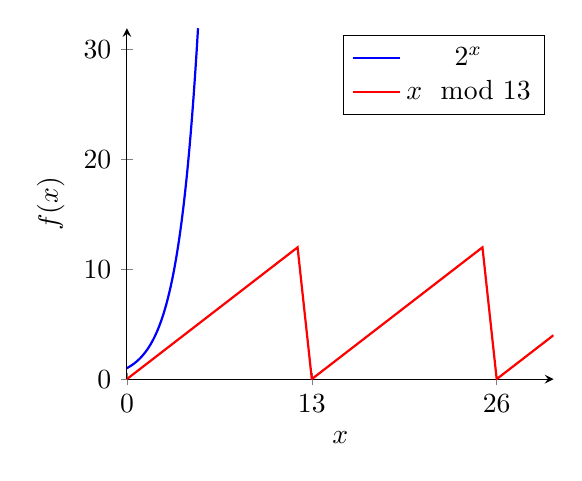
\begin{tikzpicture}
\begin{axis}[xmin=0,
            xmax=30,
            axis lines=left,
            xlabel=$x$,
            ylabel=$f(x)$,
            width=7cm,
            xtick={0,13,26}]
    \addplot[samples=100,color=blue,thick]{2^x};
    \addlegendentry{$2^x$};

    \addplot[color=red,thick] coordinates {
        (0,0) (1,1) (2,2) (3,3)
        (4,4) (5,5) (6,6)
        (7,7) (8,8) (9,9)
        (10,10) (11,11) (12,12)
        (13,0) (14,1) (15,2)
        (16,3) (17,4) (18,5)
        (19,6) (20,7) (21,8)
        (22,9) (23,10) (24,11)
        (25,12) (26,0) (27,1)
        (28,2) (29,3) (30,4)
    };
    \addlegendentry{$x\mod 13$}
\end{axis}
\end{tikzpicture}
\end{center}

\begin{flushleft}
Dieses Verhalten liegt in der Natur des Modulos.
Er gibt den Rest beim teilen durch eine bestimmte Zahl
(in unserem Fall 13) wieder.
Also gilt:
\end{flushleft}

\begin{align}   
    0&=x\mod n \\
    \Leftrightarrow x&=n\cdot m,\quad m\in\mathbb{Z}
\end{align}

\begin{flushleft}
Anders ausgedrückt, kann man eine Zahl immer restlos durch sich
selbst, oder sich selbst multiplizert mit einem ganzen Vielfachen teilen.

Für $x\mod 13=0$ existieren also unendlich viele Lösungen,
eben alle $x=13\cdot m$ mit $m\in\mathbb{Z}$.

Demnach hat die Gleichung $A=g^a\mod p$ auch unendlich viele Lösungen,
da $g^a\mod p$ nur eine andere Form von $x\mod n$ ist.

Darüber hinaus gilt außerdem auch:
\end{flushleft}

\begin{align}
    c&=x\mod n \\
    \Leftrightarrow x&=n\cdot m+c,\quad m\in\mathbb{Z}
\end{align}

\begin{flushleft}
Betrachtet man also die abgefangenen Werte, gilt folgendes:
\end{flushleft}

\begin{align}
    8&=2^a\mod 13 \\
    \Leftrightarrow 8&=x\mod 13 \\
    \Leftrightarrow x&=13n+8,\quad n\in\mathbb{Z} \\
    \Leftrightarrow 2^a&=13n+8 \\
    \Leftrightarrow \ln{2^a}&=\ln{13n+8} \\
    \Leftrightarrow a\ln{2}&=\ln{13n+8} \\
    \Leftrightarrow a&=\frac{\ln{13n+8}}{\ln{2}}
\end{align}

\begin{flushleft}
Diese Gleichung zeigt relativ gut, wie schwer es ist den diskreten Logarithmus
zu berechnen. Obwohl $n\in\mathbb{Z}$ ist, $n$ also jede ganze Zahl im Interval $]-\infty,\infty[$
annehmen kann, existiert nur ein Wert für $n$, der zu dem richtigen Wert für $a$ führt.

Hier wird $a=3$ für $n=0$.
\end{flushleft}
\end{document}
